%%%%%%%%%%%%%%%%%%%%%%%%%%%%%%%%%%%%%%%%%
% Engineering Calculation Paper
% LaTeX Template
% Version 1.0 (20/1/13)
%
% This template has been downloaded from:
% http://www.LaTeXTemplates.com
%
% Original author:
% Dmitry Volynkin (dim_voly@yahoo.com.au)
%
% Revisions:
% TEC 5-29-2014 Updated for MATH 605 and OENG 644
%
% License:
% CC BY-NC-SA 3.0 (http://creativecommons.org/licenses/by-nc-sa/3.0/)
%
%%%%%%%%%%%%%%%%%%%%%%%%%%%%%%%%%%%%%%%%%

%----------------------------------------------------------------------------------------
%	PACKAGES AND OTHER DOCUMENT CONFIGURATIONS
%----------------------------------------------------------------------------------------

\input{packages_DocConfigs}

%----------------------------------------------------------------------------------------
%	HEADER INFORMATION
%----------------------------------------------------------------------------------------

\fancyhead[r]{\begin{tabular}{L{3cm} R{3cm} | L{3cm} R{5cm}} % The header is a table with 4 columns
\textbf{Author}   & Tim Coon & \textbf{Page}         & \thepage/\pageref{LastPage} \\
\textbf{Date}      & 12/02/14 & \textbf{Course}      & AERO 899 PS \\
\textbf{Description} & Qual Q\#4     & \textbf{Reference} & Cobb \\
\end{tabular}}

%----------------------------------------------------------------------------------------

\begin{document}
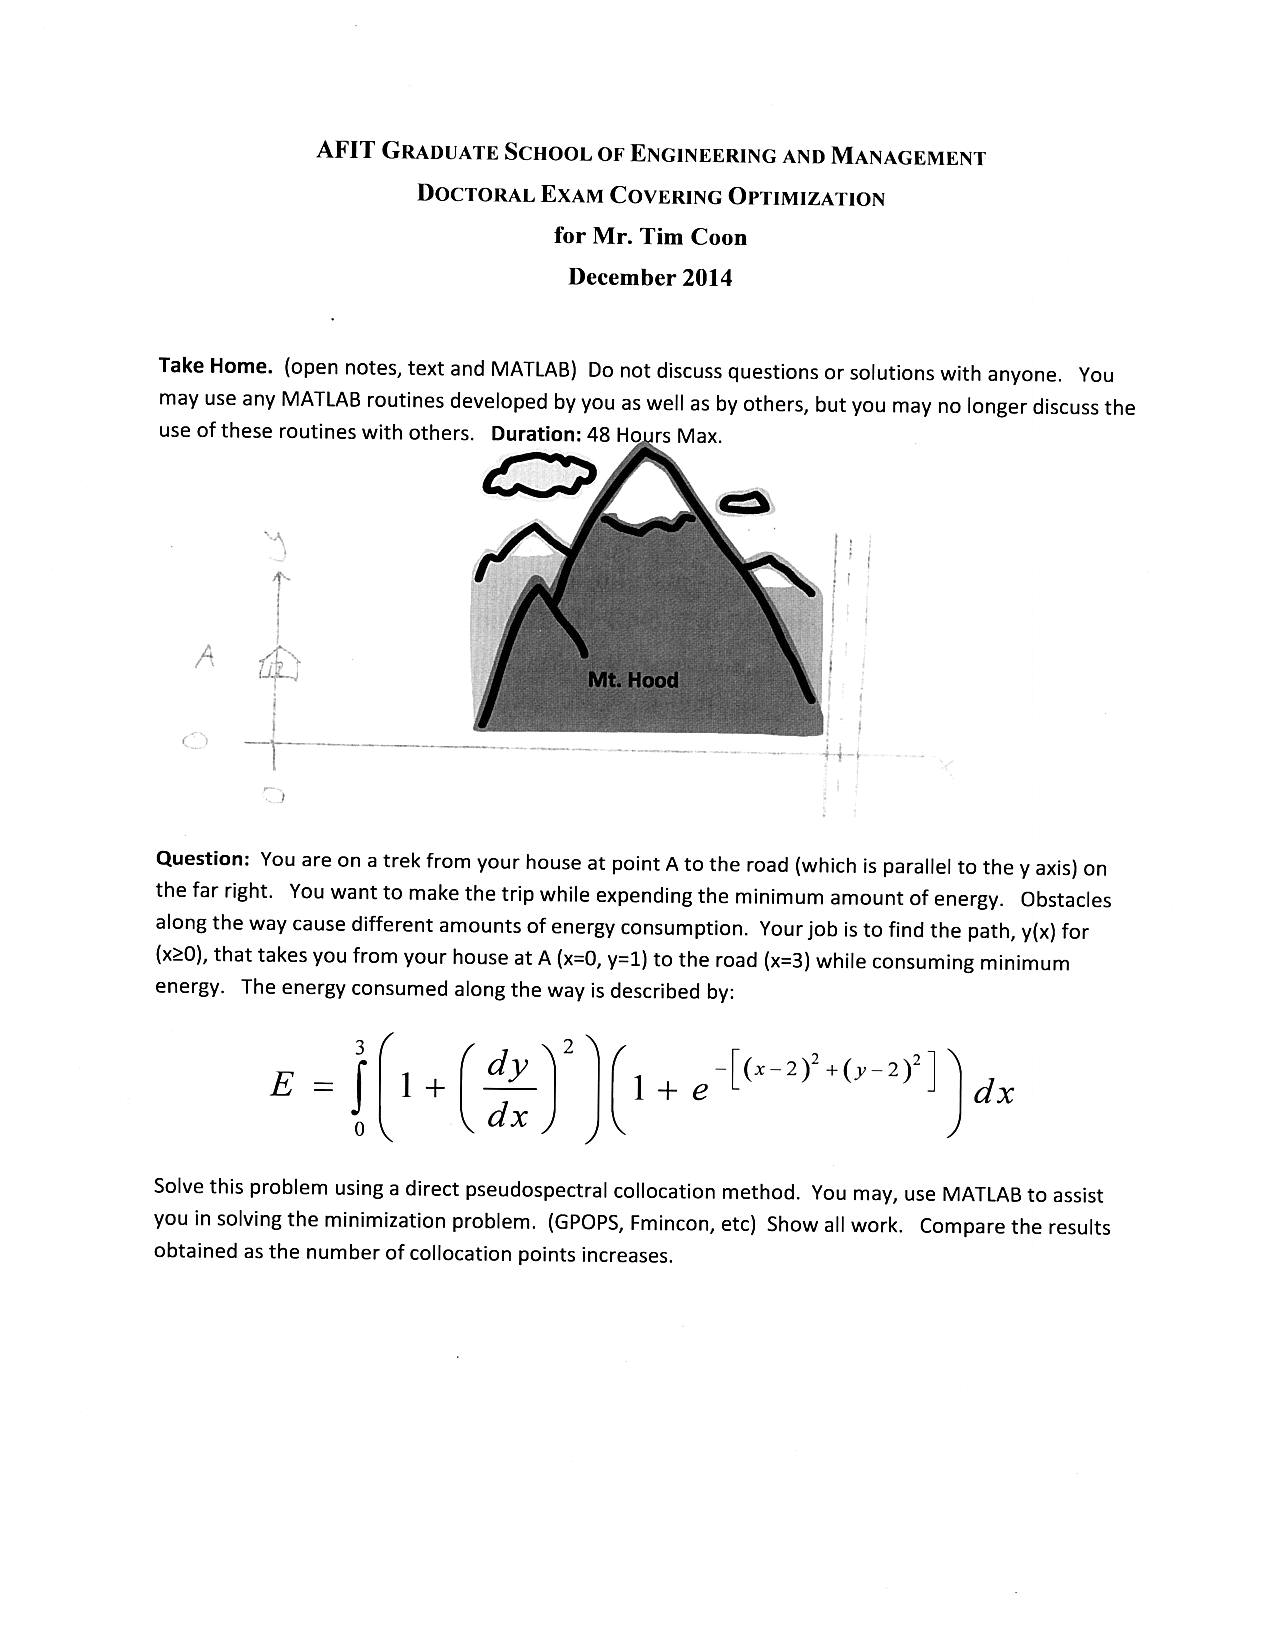
\includepdf[pages={1}]{Q4_AERO899_ProblemStatement.pdf}


\AddToShipoutPicture{\BackgroundStructure} % Set the background of each page to that specified above in the header information section

%----------------------------------------------------------------------------------------
%	DOCUMENT CONTENT
%----------------------------------------------------------------------------------------

\section*{Description and Comparison}

The min energy problem is solved using the x-position as the independent variable, rather than time. Because the integrand of the cost function is strictly positive and regular, it is unlikely for a minimum energy path to double back in the x-direction, so using x-position as the independent variable is acceptable. Evaluating the cost is more simple because the integrand of the cost functional is taken with respect to the x-direction. The MATLAB\textsuperscript{\copyright} code utilizes GPOPS-2\textsuperscript{\copyright}, Ver. 2.0 to solve the optimal control problem as follows.

\subsection*{Optimal Control Problem}

Find the control, \textbf{u}, in the set of admisible controls, \textbf{U}, that minimizes the following cost functional

\begin{equation}		% eq:cost
\label{eq:cost}
\min_{\bf\/{u}\in\bf{U}}\;\; 
E=\int_{0}^{3} \left[ 1+\left(\frac{dy}{dx}\right)^2 \right] \left[1+\exp\left(-\left[(x-2)^2+(y-2)^2\right]\right)\right]
\end{equation}

subject to the dynamic constraint
\begin{equation}
	y\prime = u
\end{equation}

where the control is
\begin{equation}
\label{eq:controls}
	u = \frac{dy}{dx}
\end{equation}

with the boundary conditions,
\begin{subequations}		% eq: BCs
\label{eq:boundaryconditions}
\begin{align}
	x0 &= 0 && y(x0) = 1 \\
	xf &= 3 && y_{min}\leq y(xf)\leq y_{max}
\end{align}
\end{subequations}

\subsection*{Solution}
The MATLAB\textsuperscript{\copyright} code and plots are attached. In the figure, solutions determined using a different number of collocation points and mesh intervals are plotted along with the "energy terrain" of the area. Neither the path nor the cost change significantly with the number of collocation points or the number of mesh intervals. The optimal path is reasonable as it moves toward the lowest energy area at the base of the mountain without making significant trajectory changes (${\frac{dy}{dx}}$). The choice of $x$ as the independent variable is further verified because the optimal control vector (the slope) does not approach the user-defined limits on either end ($u_{min}=-10$, $u_{max}=10$).

\subsection*{Furthermore}
I removed the control contribution to the cost functional, Equation~\eqref{eq:newcost} and the results vary more significantly with the number of collocation points.
\begin{equation}		% eq:newcost
\label{eq:newcost}
\min_{\bf\/{u}\in\bf{U}}\;\; 
E=\int_{0}^{3} \left[1+\exp\left(-\left[(x-2)^2+(y-2)^2\right]\right)\right]
\end{equation}

% \ClearShipoutPicture
% 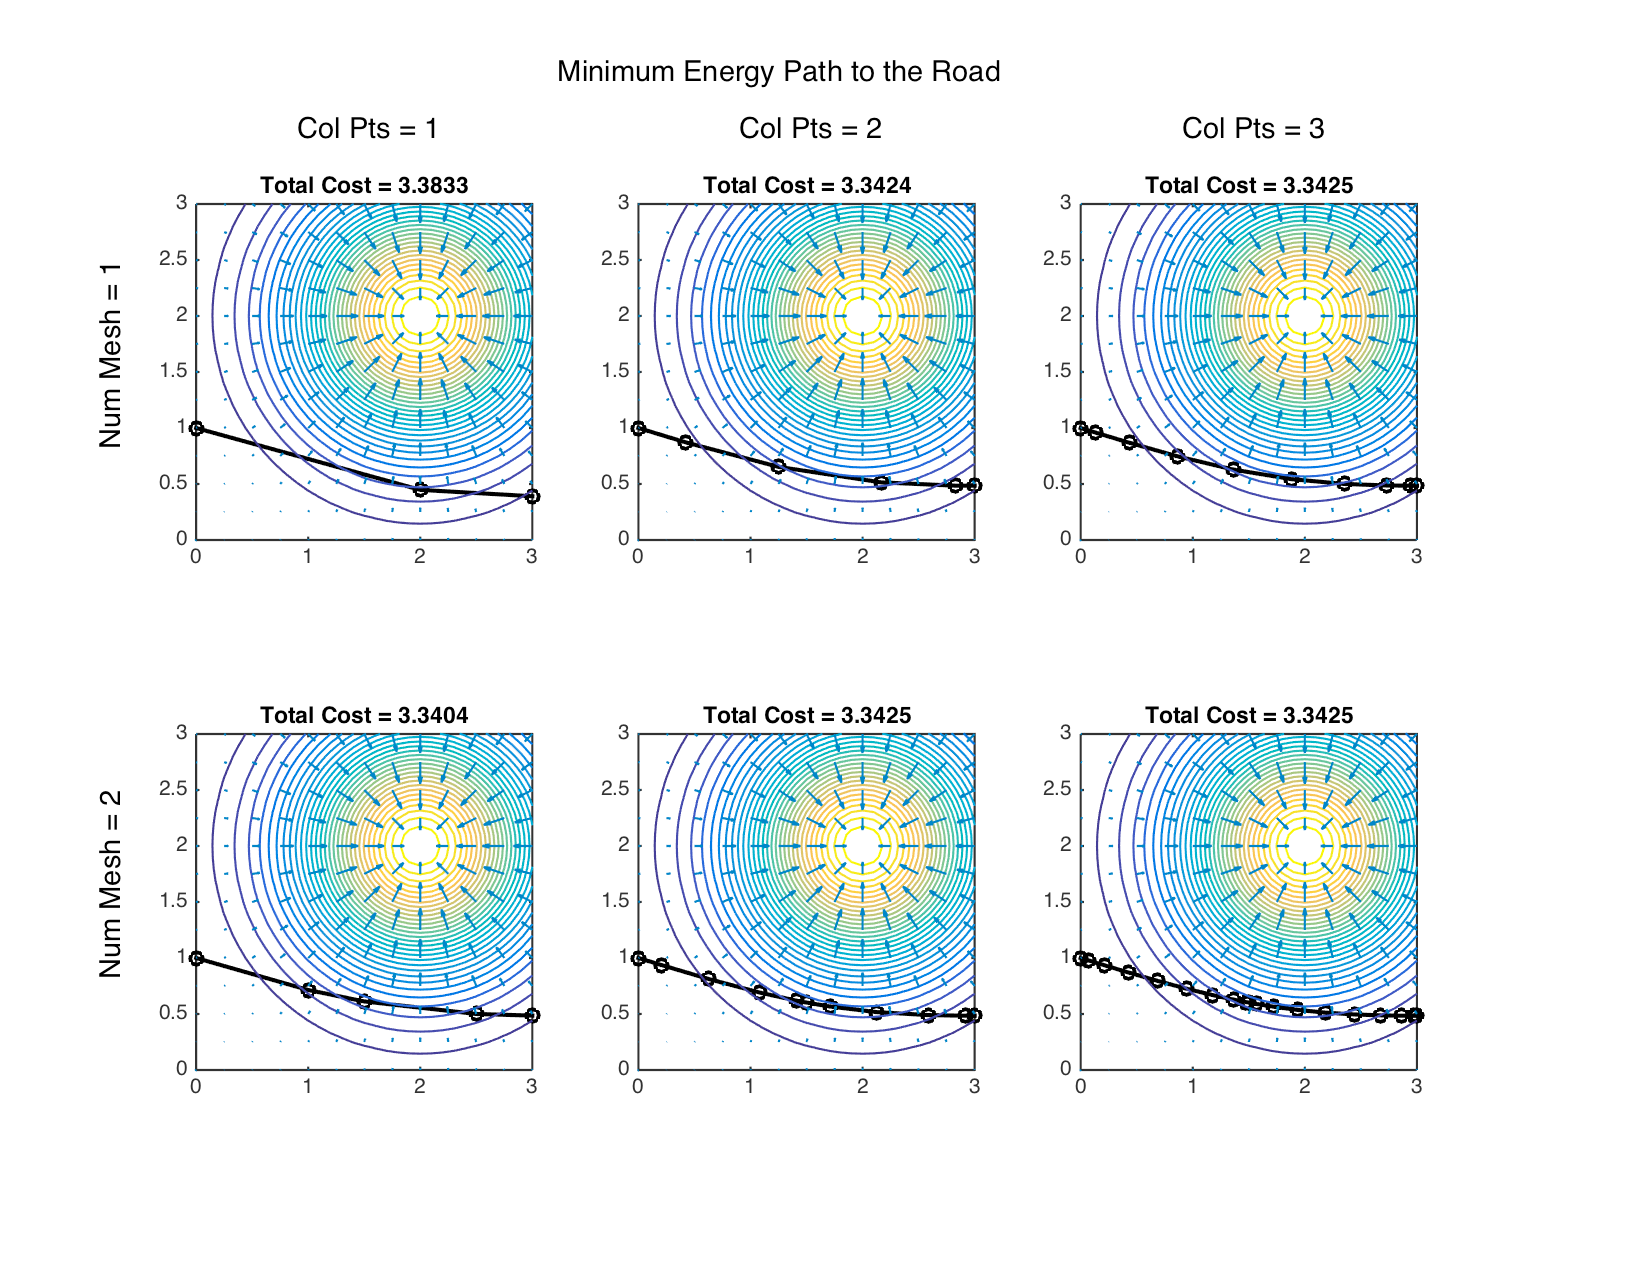
\includepdf[pages={1}]{../"Q4 PDFs"/Q4_Plots.pdf}

%----------------------------------------------------------------------------------------

\end{document}